\section{UM Tube Production}
	\subsection{Construction Process}
		\begin{frame}{Overview}
			\begin{itemize}
				\item In order to supplement supply being recieved from Michigan State University, UM started it's second wave of tube construction in November 2022.
				\item 4-5 full time workers for construction and testing, 3 part time students for additional testing. 
				\item Goal of 1000 sMDTs constructed before 2023. Average 50 Tubes/Day. 
			\end{itemize}
		\end{frame}
		\begin{frame}{Construction and Testing}
			\begin{figure}
				\centering
				\begin{subfigure}[c]{0.4\pdfpagewidth}
					\centering
					\includegraphics[width=0.5\pdfpagewidth]{TubeProduction.png}
				\end{subfigure}
				~
				\begin{subfigure}[c]{0.4\pdfpagewidth}
					\centering
					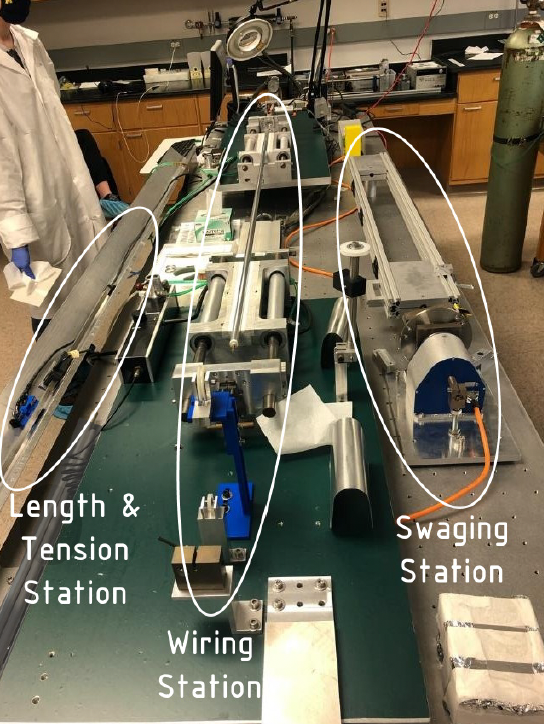
\includegraphics[height=0.4\pdfpageheight]{TubeProductionAlternateView.png}
				\end{subfigure}
			\end{figure}
		\end{frame}
		\begin{frame}{sMDT QA/QC Tests}
			\begin{figure}
				\begin{subfigure}[c]{0.4\pdfpagewidth}
					\centering
					\hyperlinktarget{DCExtra}{DC}{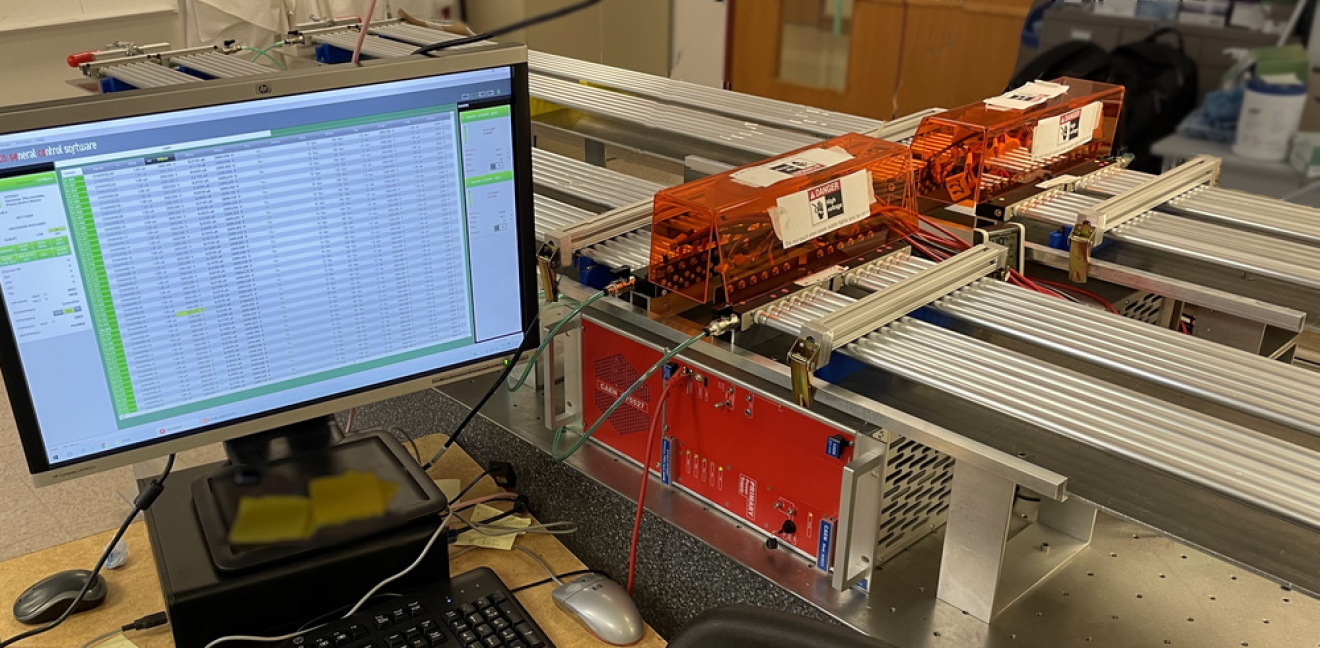
\includegraphics[width=0.7\textwidth]{CAENForDC.png}}
					\caption{Dark Current Testing setup.}
				\end{subfigure}
				\begin{subfigure}[c]{0.4\pdfpagewidth}
					\centering
					\hyperlinktarget{LeakRateTubesExtra}{LeakRateTubes}{\includegraphics[width=0.5\textwidth]{LeakDetector.png}}
					\caption{Helium Leak Testing Setup}
				\end{subfigure}
			\end{figure}

			\begin{figure}
				\centering
				\hyperlinktarget{TensionExtra}{TensionPhoto}{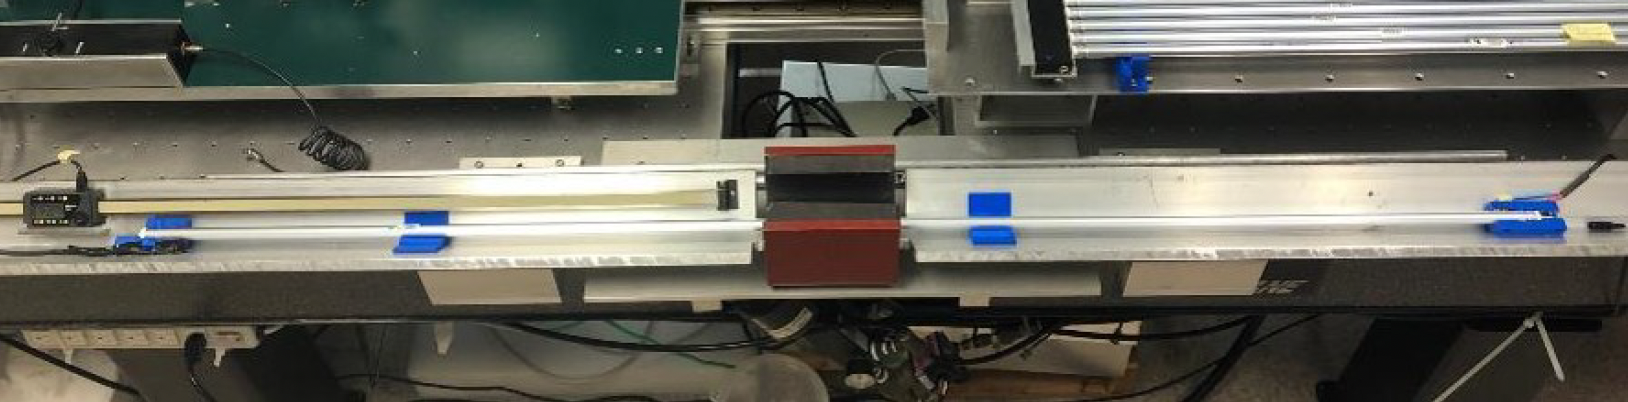
\includegraphics[width=0.6\textwidth]{TensionStation.png}}
				\caption{Tension Testing Setup}
			\end{figure}
		\end{frame}
		\begin{frame}{Results}
			\begin{itemize}
				\item Completed after 32 working days in December 2022 with 1,359 tubes total. 
				\item Constructed sMDTs still undergoing QA/QC. 
				\item 19 total failed QA tests. (Failure Rate of 1.8\%)
			\end{itemize}
		\end{frame}



